\chapter{User documentation}
\label{ch:user-documentation}

The purpose of this project is to propose and implement a system for object
localization using a stereo vision -- two cameras. The system computes relative
position of the cameras to each other using a calibration pattern. Then the user
selects the object to track. Different algorithms can be used for tracking.
The tracking algorithms available are detection-based and also sequence-based.
When the object is found in the view of the both cameras, a position in three
dimensional space is estimated. 
This part of the documentation is focused on the end user. We introduce
installation details and manual for program usage.

\section{Installation guide}
This section documents the process of downloading until running the program.

\subsection{Downloading the code}
The code is available at \url{https://github.com/JankaSvK/thesis}.

\subsection{Hardware requirements}
The software was tested on a system with Intel(R) Core(TM) i5-7300HQ CPU
(2.50GHz, 2496 MHz, 4Core), 16GB RAM running Microsoft Windows 10 Enterprise.
Minimal requirements are lower, but the computation power reflects on frequency
of getting localization results. Also, we tested the program on the Ubuntu
16.04.

Two cameras are needed. We tested using a Logitech V-U0018 and Genius
Slim 1322AF. A laptop camera may be used too. Requirements for the cameras
are at least $640\times320$ px resolution and 20 FPS. We advise to turn off the
autofocus, as it changes the focal length.

\subsection{Dependencies}
The following packages are required to run the application. We also provide
versions of packages used to create and test our implementation.

\begin{center}
\begin{tabular}{l l}
	package	&	version 	\\ \hline
	Python	&	3.4.0 		\\
	NumPy	&	1.13.3 		\\
	OpenCV-contrib	&	3.4.0 	\\ 
	Matplotlib &	2.1.1 		\\
	Tkinter	&	8.6 		\\
	PIL (with ImageTk module)	&	1.1.7 		\\
	dlib	&	19.10.0
\end{tabular}
\end{center}

You can easily check the installed versions by running \verb+checkVersions.py+ in
the directory \verb+helpers/+, which is located in the root of the repository.

\section{First run}

In the folder \verb+program/+ we find an entry point for our application
\verb+Main.py+. The text in this chapter is written with assumption that
current directory is the directory \verb+program/+. After starting the
application a window will show up (displayed in Figure \ref{fig:application}).
With no options provided, the program will run on the first two cameras
available.

\begin{figure}
	\frame{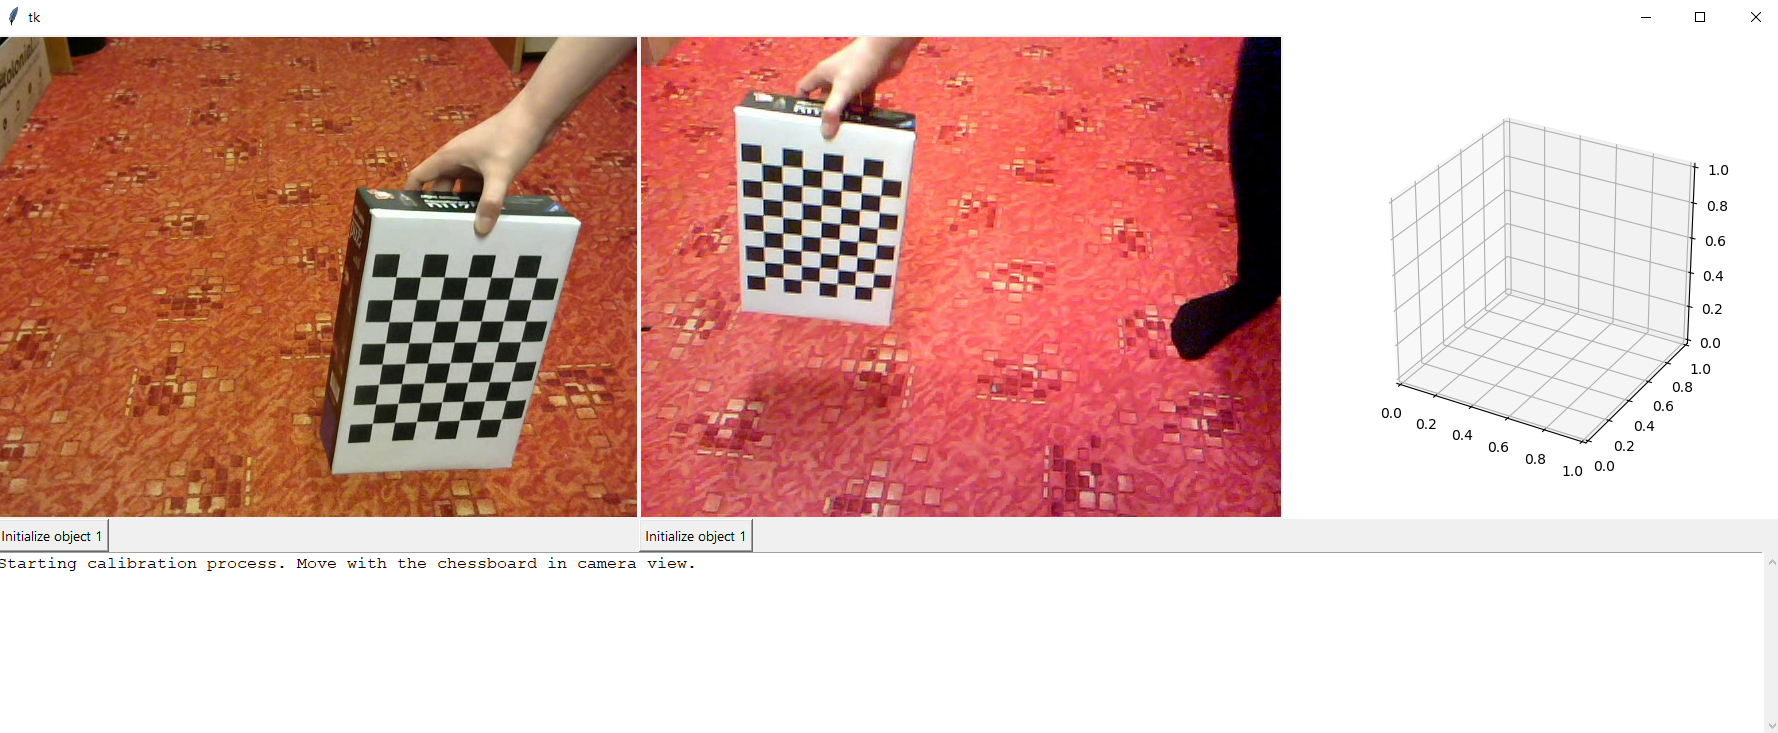
\includegraphics[width=\linewidth]{img/application.png}}
	\caption{Application window}
	\label{fig:application}
\end{figure}

\subsection{Calibration}
As a first step, calibration is expected. We need a calibration pattern --
chessboard (example in the Figure \ref{fig:chessboard}), which could be
printed. For given chessboard, edit values in \verb+program/Config.py+. Change
the value of \verb+chessboard_inner_corners+ to a number of \emph{inner}
corners of your chessboard. For example, classic chessboard 8 $\times$ 8
squares has only 7 $\times$ 7 inner corners, so we enter a tuple \verb+(7, 7)+
as a number of inner corners. Also change \verb+chessboard_square_size+ to the
size of your square in millimeters. It is important to check, if printed
chessboard has squares, not rectangles, since the printer can slightly scale
the image while preprocessing for printing.  Moreover, calibration assumes it
is a planar object, so glue it to the box or another solid object.

For calibration we have to provide a rich set of views of the chessboard. It is important
to move with it and to capture it from various angles, distances and in different
parts of the image. A richer set of views increases robustness of the calibration.

After each successful calibration step you will be notified in the console.
After successful stereo calibration, estimated distance between the cameras
will be printed. If it does not correspond to the reality, consider
a recalibration. If it still did not helped, the user can increase the number of
images needed for calibration in the configuration file (be careful, the computation
time may increase).

If the calibration finished successfully, the calibration results will be
automatically saved in \verb+program/calib_results/+. The files will be saved
into three directories, regarding if it is stereo or mono calibration. In case
of mono calibration, it will be stored in the folder of corresponding camera.
The hierarchy is displayed in the Figure \ref{fig:hierarchy-calib}. The naming
convention for these files is
\verb+{year}-{month}-{day}-at-{hour}-{minute}.json+, where the date and time
specify the moment when the calibration finished.

\begin{figure}
\dirtree{%
.1 calib{\_}results/.
.2 stereo{\_}calib{\_}results/.
.2 1/.
.2 2/.
 }
 \caption{Hierarchy of the directory with saved calibration results}
 \label{fig:hierarchy-calib}
\end{figure}

\subsection{Selecting the objects}
After successful calibration (calibrated with chessboard, or loaded from a
file), the user can initialize the trackers. Under each view of the camera, a button
for each object is located.

For tracker initialization, click on the button. The next two clicks in the
view of the camera, will specify the bounding box for the object. After
initializing trackers in both cameras, localization will automatically start.

If the tracker lost the object, the message is displayed in the camera
view. Note that, not all trackers are able to recognise losing the object.

\subsection{Localization}

After initialization of the trackers, localization will start automatically.
The results are displayed in the graph on the right. We can rotate the graph by
grabbing it by mouse in its window. The dot represents the current position and
the line represent the trajectory.

Results from localization are automatically saved at the end of the program in
\verb+program/localization_data/+. The naming convention for the files includes
the date and time, when was the program closed, i.e it has following form:
\verb+{year}-{month}-{day}-at-{hour}-{minute}-{object_id}.json+.

Saved localization data consists of the four columns separated by tabs. Each
line represents successful localization. In the first column is the time. In the
rest three columns coordinates are stored (x, y, z).

\section{Extras}

Different options may be passed to the program (\ref{code:options}). In case no option
is passed, the program runs on first two available cameras. Firstly, calibration for
each camera is done and then stereo calibration. As a tracker \verb+KCF+ is used by default.

\begin{figure}
\lstset{basicstyle=\ttfamily\footnotesize,breaklines=true,frame=lrtb}
\lstinputlisting[label={code:options}, caption={Available options}]{options.txt}
\end{figure}

\subsection{Notes for options}
\begin{itemize}
\item\emph{Videos} -- only AVI formats are accepted.
\item\emph{Trackers} -- as \verb+TRACKER+ may be used a name of implemented tracker.
Allowed tracker names are: 
\verb+BOOSTING+,
\verb+CORRELATION+,
\verb+HSV+,
\verb+KCF+,
\verb+MEDIANFLOW+,
\verb+MIL+,
\verb+MOSSE+
\verb+PATTERNMATCHING+,
\verb+SIMPLEBACKGROUND+,
\verb+TLD+.
\item\emph{Calibration results} -- calibration results from previous runs may be
used by specifying path to the file.
\item\emph{Chessboard} -- the expected format is for example
\verb+--chesboard=7,8,22+, where the first two number specify number of inner
corners and third is the length of the square side in millimeters.
\end{itemize}

\subsection{Capturing the videos} 

We provide additional script to capture and save videos. The script will
automatically capture video from all available cameras and save it into
\verb+captured_videos+. The capturing can be exited by pressing the key "q".
The script is available in \texttt{helpers/video\_capture.py} from the root
directory of the repository.  

\subsection{Sample scenarios}

\texttt{python3 Main.py} -- runs the application on first two available cameras
\newline
\texttt{python3 Main.py --video1=path/file.avi --video2=path/file.avi} -- runs the application on the videos instead of the cameras
\newline
\texttt{python3 Main.py --tracker=CORRELATION} -- use a correlation tracker
\newline
\texttt{python3 Main.py --chessboard=7,8,22} -- using a chessboard pattern with $7\times8$ inner corners, each has 22 millimeters long side
\newline
\texttt{python3 Main.py -o2} -- setting to track two objects
